\subsection{Cell Processor Comparison}
\label{subsec:dataset_info}
See \autoref{chart:cell_density_A} and \autoref{chart:cell_density_B} for the results\footnote{All benchmarks were run with double precision. The thread block cell processor was run with dedicated shared memory, the warp block cell processor without.}. The specified warp count always refers to the used warps per thread block.

\begin{sidewaysfigure}
\centering
\subfloat[warp block processor]{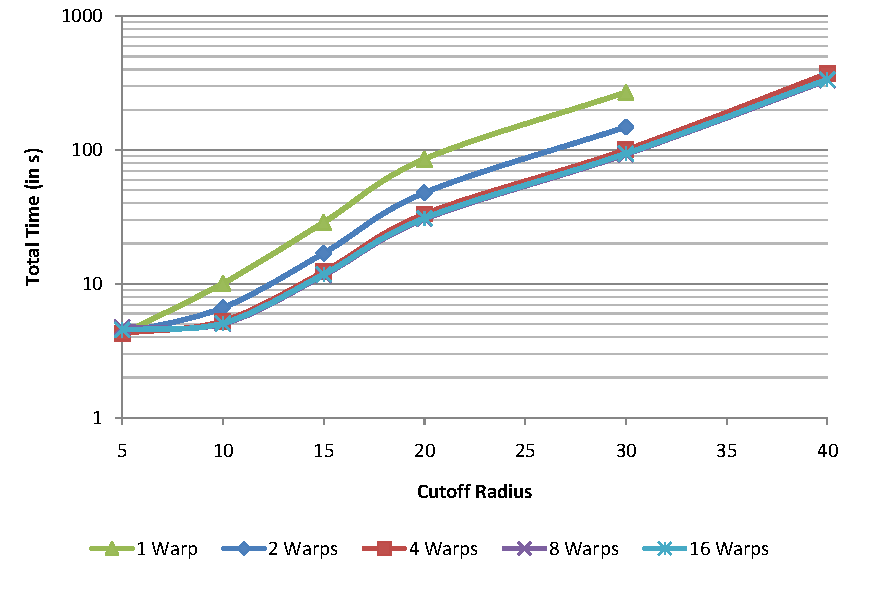
\includegraphics[width=0.5\textwidth]{plots/cell_density_wbdp.pdf}}
\subfloat[thread block processor]{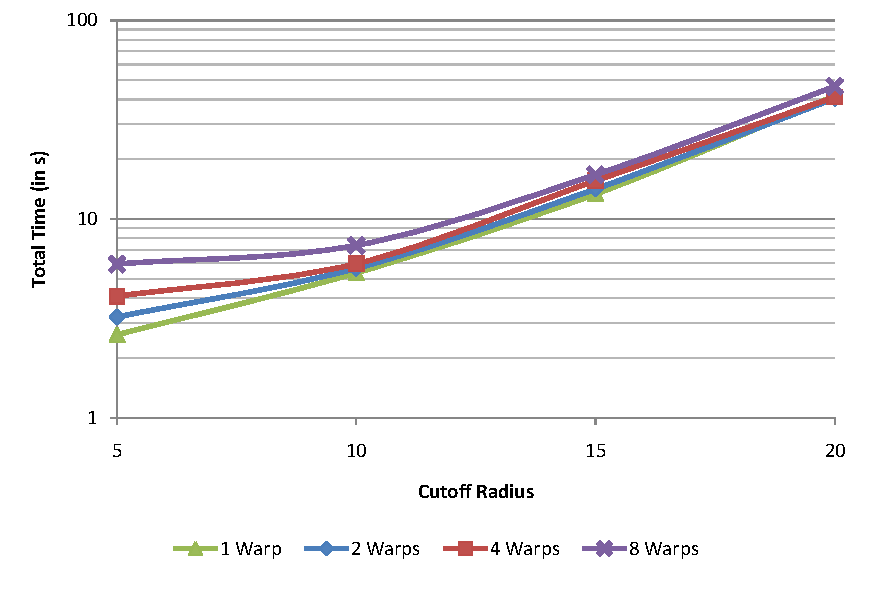
\includegraphics[width=0.5\textwidth]{plots/cell_density_dp.pdf}}\\
\subfloat[summary chart]{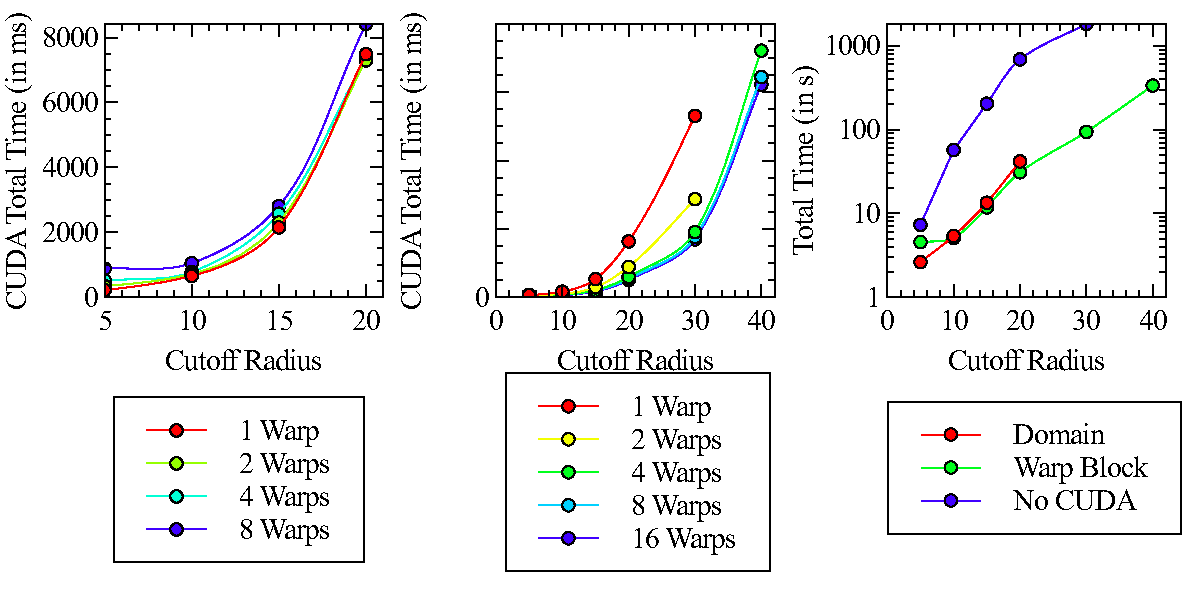
\includegraphics[width=0.5\textwidth]{plots/cell_density.pdf}}
\caption{benchmark results for different cutoff radii on workstation A (dataset: \filename{lj\_80000})}
\label{chart:cell_density_A}
\end{sidewaysfigure}
\begin{sidewaysfigure}
\centering
\subfloat[warp block processor]{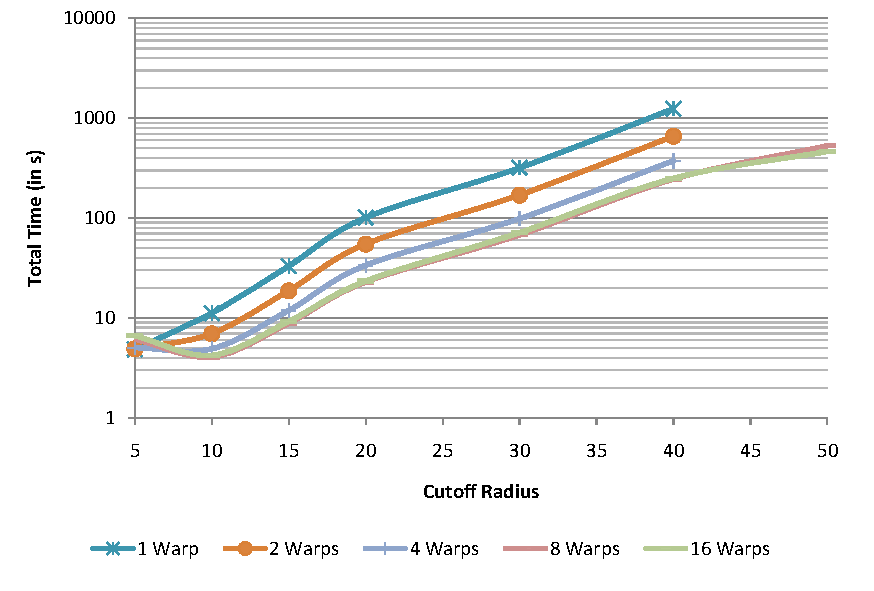
\includegraphics[width=0.5\textwidth]{plots/cell_density_tesla_wbdp.pdf}}
\subfloat[thread block processor]{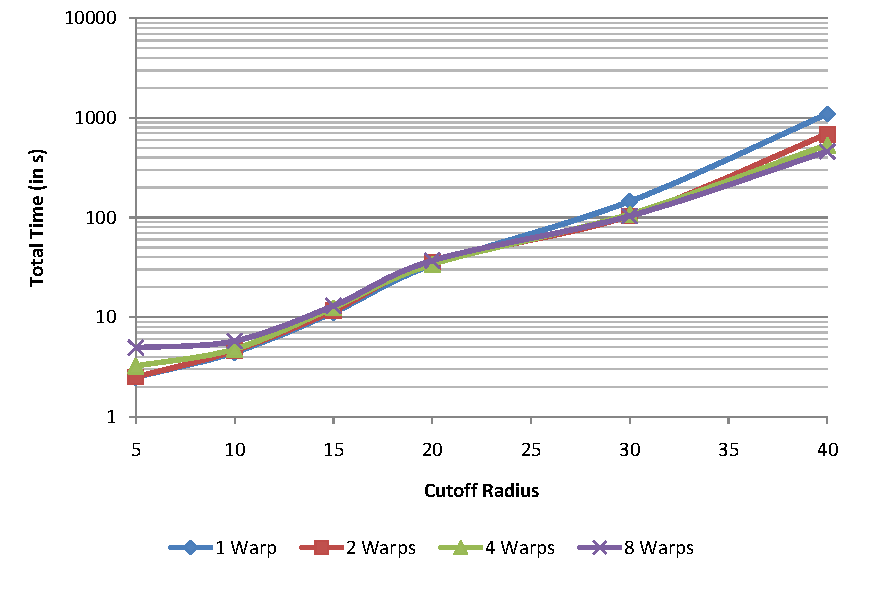
\includegraphics[width=0.5\textwidth]{plots/cell_density_tesla_dp.pdf}}\\
\subfloat[summary chart for \filename{lj3d1\_lj2d1\_50000}]{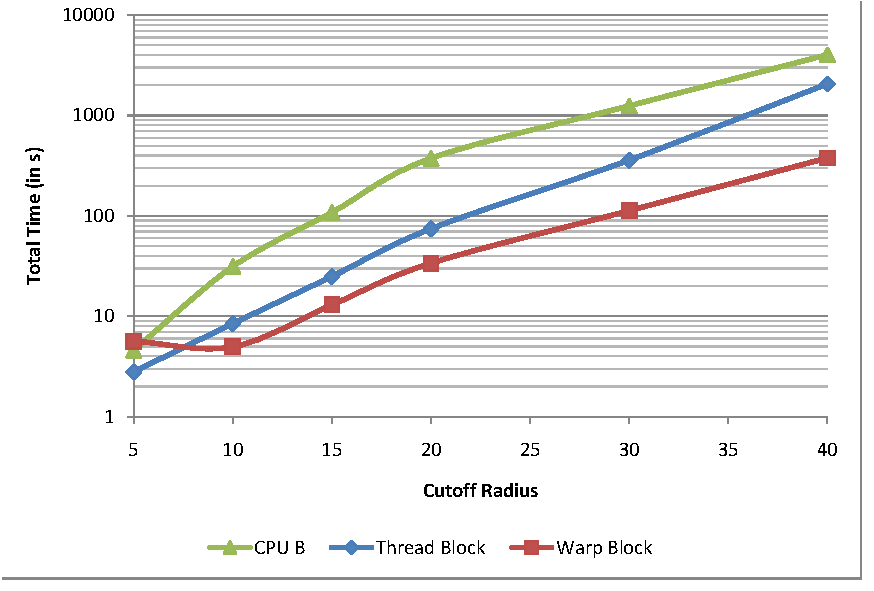
\includegraphics[width=0.5\textwidth]{plots/cell_density_tesla_mix.pdf}}
\subfloat[summary chart for \filename{lj\_80000}) ]{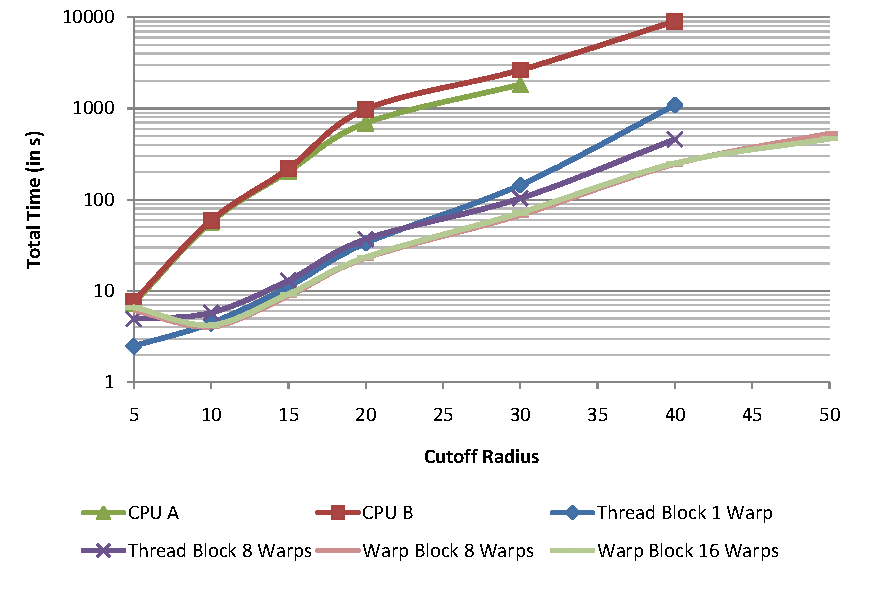
\includegraphics[width=0.5\textwidth]{plots/cell_density_tesla.pdf}}
\caption{benchmark results for different cutoff radii on workstation B}
\label{chart:cell_density_B}
\end{sidewaysfigure}

The \filename{lj\_80000} dataset consists of that many molecules with a single Lennard-Jones center.
The \filename{lj3d1\_lj2d1\_50000} dataset consists of a mix of molecules with 3 Lennard-Jones centers and 1 dipole and molecules with 2 Lennard-Jones centers and 1 dipole.
The \filename{lj3d1\_50000} dataset only consists of molecule of the former kind.

The charts are plotted against varying cutoff radii. This means that the molecule material density remains constant and only the varying cutoff radius is used to increase the number of molecules in the cells (the length of cell is exactly the cutoff radius).

\autoref{chart:molecule_count_histogram} shows the molecule counts per cell for the different datasets and different cutoff radii.
The y-axis shows the molecule count. The width of the bars represents the ratio of the number of cells with a given molecule count to the total number of cells.

You should keep in mind that number of cells decreases with increasing cutoff radius: for a cutoff radius of 50 there are only 27 cells (1 inner cell and 26 halo cells), while for a cutoff radius of 5 there are many cells.

As you can see, the higher the cutoff radius, the higher the average number of molecules and the smaller the variance in the molecule counts per cell.

\begin{figure}
\centering
\subfloat[\filename{lj\_80000}]{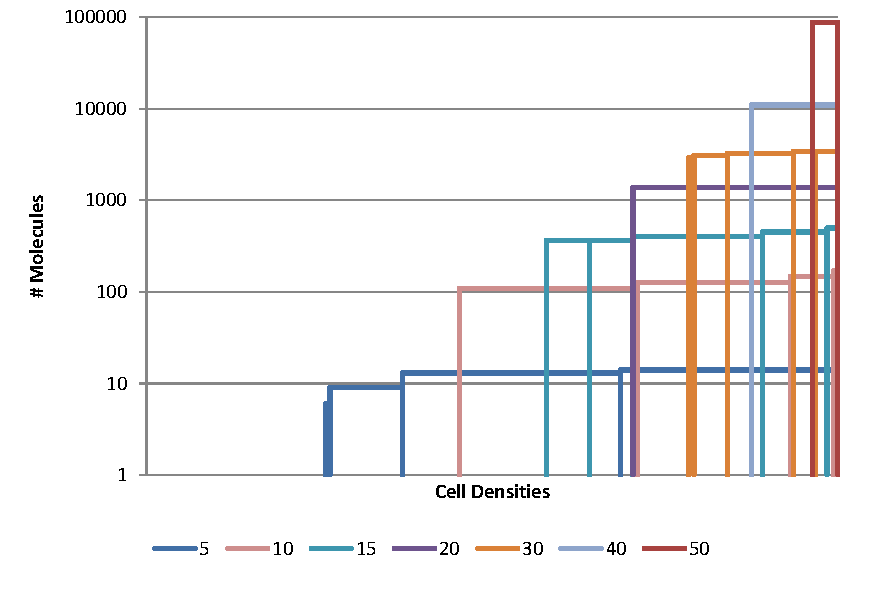
\includegraphics[width=0.5\textwidth]{plots/lj_histogram.pdf}}
\subfloat[\filename{lj3d1\_50000}/\filename{lj3d1\_lj2d1\_50000}]{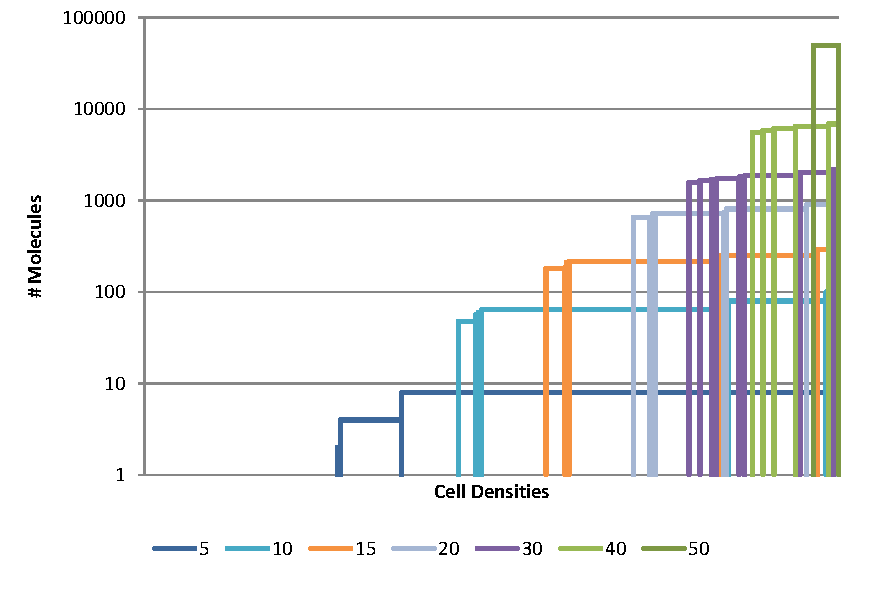
\includegraphics[width=0.5\textwidth]{plots/mix_histogram.pdf}}\\
\caption{cell molecule count histogram (for varying cutoff radii)}
\label{chart:molecule_count_histogram}
\end{figure}

\paragraph{Thread Block Cell Processor}
Only for big cutoff radii the thread block cell processor starts scaling at all. For small radii $<= 20$ using only 1 warp per thread block always is fastest. Actually using many warps per thread block is significantly slower than just using 1 warp. The reason for this negative scaling is the low cell density for small cutoff radii. If many cells have less molecules than the warp size, even some threads of only one warp are already idling. Adding more warps just adds more idle threads that need to be scheduled. Since there is a limit for resident threads on an SM, this clogs the SMs.
However, for big cutoff radii these threads will actually be put to use.

The thread block cell processor is inflexible in this regard because it always uses a fixed amount of warps per thread block for each cell or cell pair. Thus high warp counts only really work well for domains with homogenously high molecule counts per cell, whereas a warp count of 1 works best for low molecule counts per cell.

\paragraph{Warp Block Cell Processor}
This cell processor scales as expected with increasing warp counts per thread block. However, for all but the highest cutoff radii, it runs faster with 8 warps than with 16. 16 warps win with very high molecule counts per cell though.

For low cutoff radii, the additional overhead in the scheduler negates the benefits of having additional warps available for processing.

\paragraph{Summary}
The thread block processor runs best for low to mid-range cutoff radii with only 1 warp. For high cutoff radii one can use more warps.
Compared to the CPU the thread block cell processor always is faster---for mid-range cut off radii by one order of magnitude.

The warp block cell processor scales better. For low densitities, it doesn't run that well compared to a thread block cell processor with only 1 warp, but already for a cutoff radius of 10 it runs faster than the thread block cell processor and it stays this way.

Compared to the CPU and the thread block cell processor this cell processor runs fastest and scales best except for very low molecule per cell counts.

\subsection{Shared Memory versus HW Cache (Thread Block Cell Processor)}
It is possible to reduce the shared memory size from 48 to 16 KB and increase the available L1 cache per SM to 48 KB.

The thread block processor normally uses shared memory to cache molecule data that is being used.
I have tried using a bigger L1 cache and disabling the shared memory storage. The results are mixed as can be seen in \autoref{chart:shared_vs_cache}.

Using the bigger L1 cache is faster for low cutoff radii. As the molecule count per cell increases the results become mixed: using the cache is faster for the simple \filename{lj\_80000} dataset but slower for the more complex \filename{lj3d1\_50000} or \filename{lj3d1\_lj2d1\_50000} datasets.
\begin{chart}
\centering
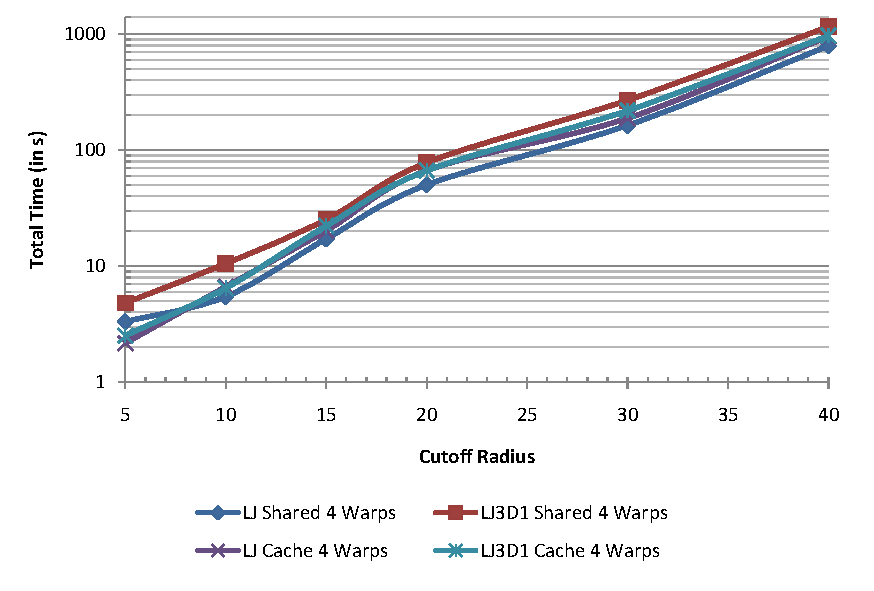
\includegraphics[width=0.75\textwidth]{plots/shared_vs_cached_tb_tesla.pdf}
\caption{shared memory vs HW cache in the thread block block cell processor (on workstation B)}
\label{chart:shared_vs_cache}
\end{chart}

\subsection{Shared Memory versus HW Cache (Warp Block Cell Processor)}
As with the thread block cell processor, there are two modes in the warp block cell processor. One uses shared memory to cache the calculated results and the other only uses an enlarged L1 cache.
As you can see in \autoref{chart:wbcp_mode_comp_tesla} there are very mixed results, too. Only results for small cutoff radii are shown because performance for the shared memory version degrades very much with higher cutoff radii.

For the warp block cell processor, everything is inverse: shared memory performs better than the HW cache for the smallest cutoff radius and worse for bigger cutoff radii.

The problem is that the additional synchronization due to locking outweighs any benefit of shared memory. When the cutoff radius is 5, only one warp is needed per cell, so no locking occurs. For bigger cutoff radii locking has a huge impact on performance\footnote{The current implementation worsens this because it tries to execute all warp blocks of a cell at once, so warps will almost always have to wait for each other.}

\begin{chart}
\centering
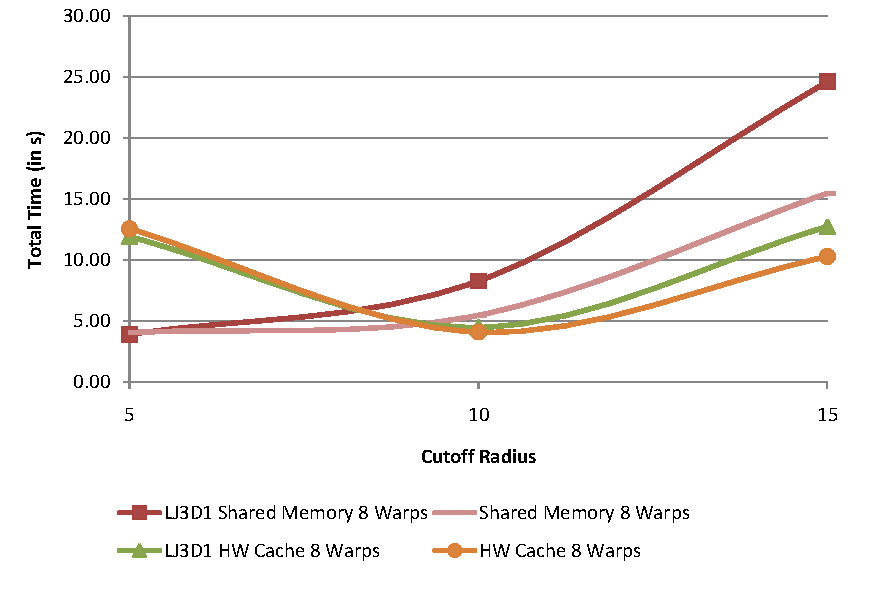
\includegraphics[width=0.75\textwidth]{plots/wbcp_mode_comp_tesla.pdf}
\caption{shared memory vs HW cache in the warp block cell processor (workstation B)}
\label{chart:wbcp_mode_comp_tesla}
\end{chart}

\subsection{Single Precision Floating Point Mode}
All the observations hold for single precision mode. Using single instead of double precision doubles the speed as you can see in \autoref{chart:float_mode_tesla}.

\begin{chart}
\centering
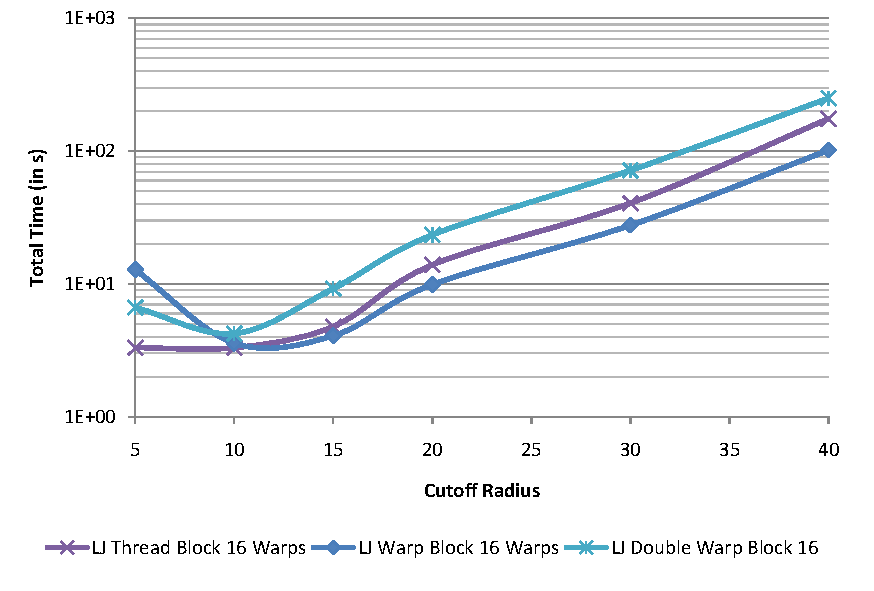
\includegraphics[width=0.75\textwidth]{plots/float_mode_tesla.pdf}
\caption{single precision floating point results}
\label{chart:float_mode_tesla}
\end{chart}

\subsection{Local and Global Error}
See \autoref{chart:error_overview} for charts that show the local and global errors. GPU potential and virial are compared to CPU ones and show the global error, whereas the RMS values show the local error between CPU and GPU calculations.

The error chart for the simple \filename{lj\_80000} dataset looks very good, but the global error is off for the more complex datasets.
For one the GPU only has a precision of 64 bits, while the FPU uses 80 bits internally.
Secondly, the dipole force and torque calculation code on the GPU is not the same as the one on the CPU in contrast to the Lennard-Jones potential code which is exactly the same.
This is due to me optimizing the code to use less variables and registers.

\begin{sidewaysfigure}
\centering
\subfloat[\filename{lj\_80000}]{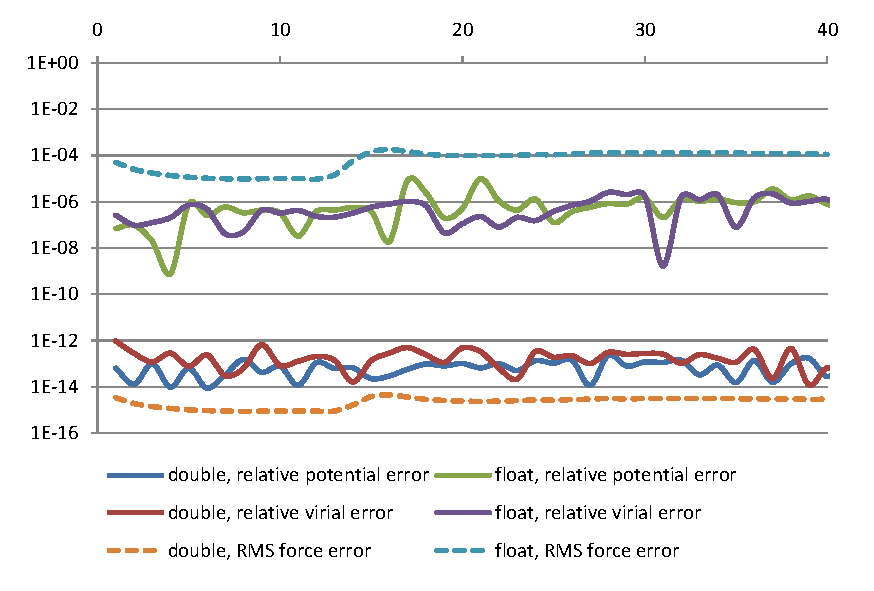
\includegraphics[width=0.5\textwidth]{plots/error_lj_tesla.pdf}}
\subfloat[\filename{lj3d1\_50000}]{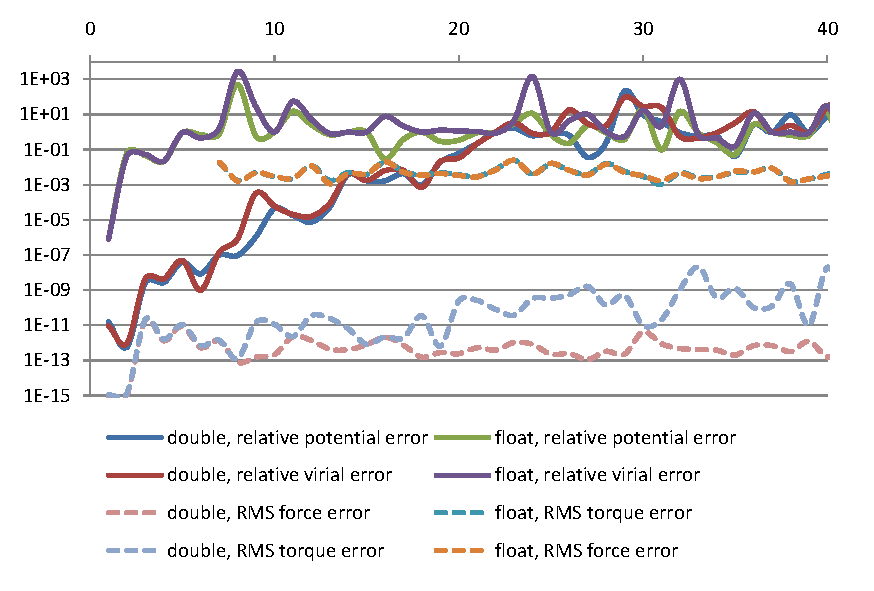
\includegraphics[width=0.5\textwidth]{plots/error_lj3d1_tesla.pdf}}\\
\subfloat[\filename{lj3d1\_lj2d1\_50000}]{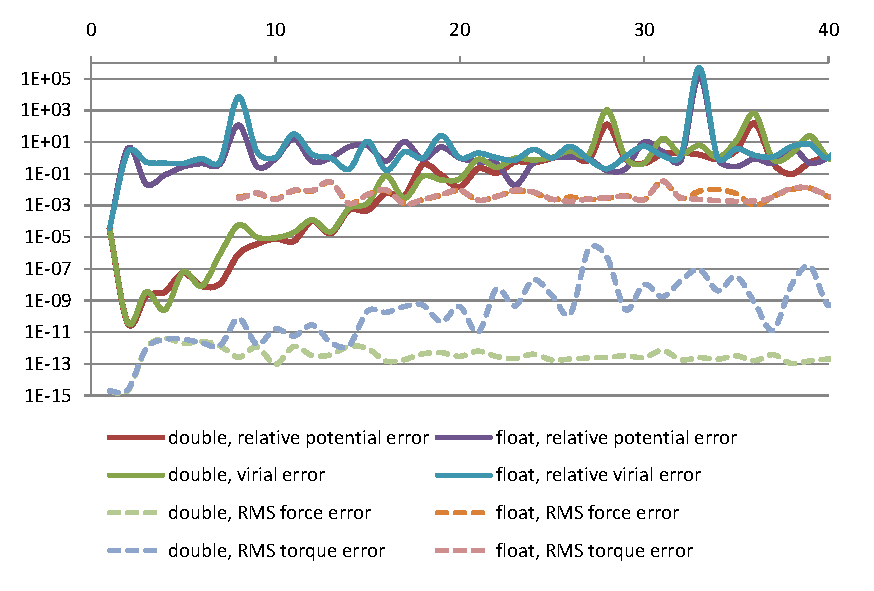
\includegraphics[width=0.5\textwidth]{plots/error_mix_tesla.pdf}}
\caption{local and global error measurements on workstation B}
\label{chart:error_overview}
\end{sidewaysfigure}